\documentclass[a4paper,11pt]{article}

% Packages
\usepackage{graphicx}
\usepackage{amsmath}
\usepackage{amssymb}
\usepackage[margin=2cm]{geometry}
\usepackage{enumitem}
\usepackage{tasks}
\usepackage{svg}

% Title info
\author{Dr Jon Shiach}
\date{Semester 1}

% Tasks package
\usepackage{tasks}
\DeclareInstance{tasks}{alphabetize-parens}{default}{
    label = (\alph*),
    label-width    = 2em,
}
\settasks{style=alphabetize-parens}

% Commands
\renewcommand{\vec}{\mathbf}

\title{Co-ordinate Geometry Exercises}

\begin{document}


\maketitle

\begin{enumerate}[label=4.\arabic*]
    \item Given the following position vectors in $\mathbb{R}^3$
    \begin{align*} 
        \vec{a} &= \begin{pmatrix} 2 \\ 1 \\ 0 \end{pmatrix}, &
        \vec{b} &= \begin{pmatrix} 1 \\ 1 \\ 0 \end{pmatrix}, &
        \vec{c} &= \begin{pmatrix} 3 \\ -1 \\ 4 \end{pmatrix}, &
        \vec{d} &= \begin{pmatrix} 5 \\ 2 \\ 6 \end{pmatrix}.
    \end{align*}
    find:
    \begin{enumerate}
        \item the equation of the line that passes through $\vec{a}$ and $\vec{b}$;
        \item the equation of the line that passes through $\vec{c}$ and $\vec{d}$;
        \item the equation of the plane which passes through $\vec{a}$, $\vec{b}$ and $\vec{c}$ lie;
        \item the equation of the plane upon which passes through $\vec{b}$, $\vec{c}$ and $\vec{d}$.
    \end{enumerate}

    \item Find the equation of the line that passes through the point with position vector $(3, 2, 1)^\mathsf{T}$ which is parallel to $2 \vec{i} + \vec{j} + 3 \vec{k}$.
    
    \item Find the equation of the plane that passes through the point with position vector $(3, 2, 5)^\mathsf{T}$ which has a normal vector $\vec{n} = (2, 1, 3)^\mathsf{T}$.
    
    \item A plane has the equation $3x - 2y + z = 10$. Identify the normal to the plane and find the co-ordinates of 2 points on the plane having $z = 2$.
    
    \item Two lines in $\mathbb{R}^3$ are defined by $\ell_1: (1 + 2t, -t, 1 + 3t)^\mathsf{T}$ and $\ell_2: (1 + 2t, 4, 7 - t)^\mathsf{T}$ respectively.
    \begin{enumerate}
        \item find the intersection of the lines or show they are skew;
        \item find the distance between the point with position vector $\vec{p} = (0, -1, 3)^\mathsf{T}$ and $\ell_1$;
        \item find the shortest distance between the lines.
    \end{enumerate}

    \item Find the point where the line $\ell:(1 + 2t, 2 + t, -1 + 4t)^\mathsf{T}$ meets the plane $6x - y - 4z = 3$. 
    
    \item Consider the diagram below that shows a plane that passes through the point $\vec{p}$ and has normal vector $\vec{n}$ and the point with position $\vec{q}$ not on the plane. 
    \begin{center}
        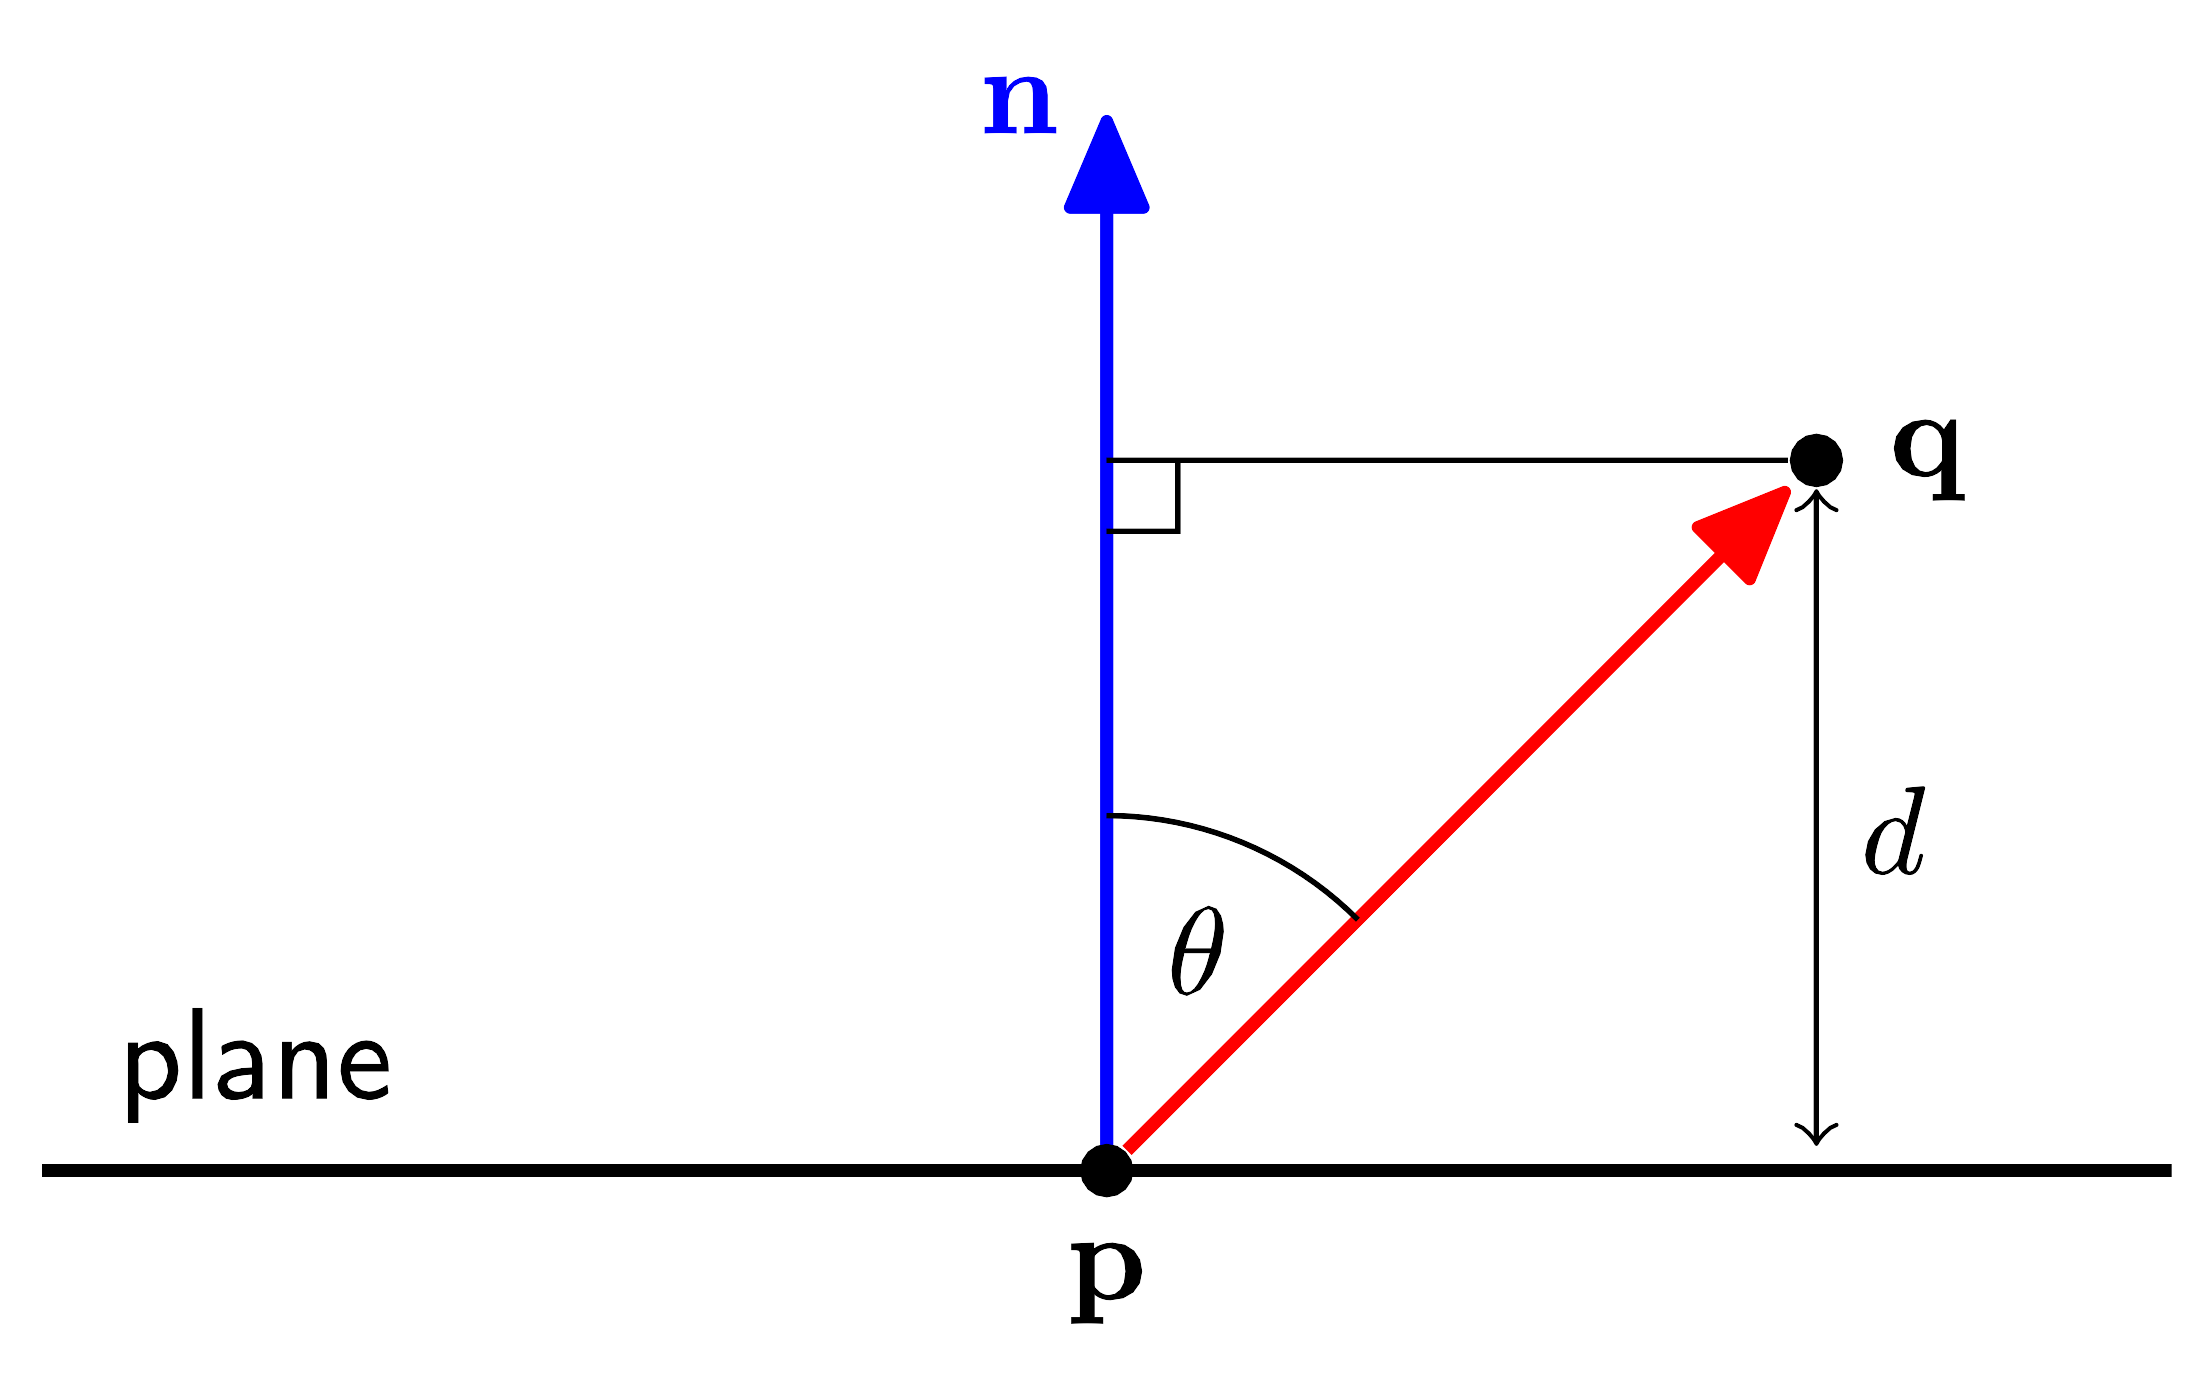
\includegraphics[width=0.4\textwidth]{images/4_point_plane_distance.png}
    \end{center}
    Using the geometric definition of a dot product, derive an expression for calculating the shortest distance between a point and a plane. Use your expression to find the shortest distance from the point with position vector $(2, 4, -3)^\mathsf{T}$ to the plane $6x - y - 4z = 3$.
\end{enumerate}

\end{document}